\chapter{Conclusioni}

Dopo aver studiato il funzionamento delle varie tecniche applicabili per eseguire un Brute Force, possiamo dire che alla stessa velocità con cui aumentano l'affidabilità dei algoritmi di criptazione delle nostre password, vengono trovati nuovi modi per decifrarli.

Come abbiamo potute vedere, le tecniche e i strumenti per eseguire questo tipo di operazioni, permettono di sfruttare diversi approcci (anche uniti tra di loro) e la potenza computazionale completa di un dispositivo, sia CPU che GPU, inoltre abbiamo potuto vedere anche tecniche che permettono di unire le potenze di calcolo di dispositivi diversi.

\section{Sviluppi futuri}

Uno dei problemi più grandi per chi attacca gli hash, è quello di incontrare algoritmi di criptazione troppo, complessi, ci sono alcuni algoritmi come : AES-256 e RSA, che per essere decriptati, richiedono una potenza di calcolo elevatissima, quasi infinitesimale, ma con l'avvenire delle nuove tecnologie e con il futuro avvento dei computer quantisci, anche questi algoritmi, potrebbere diventare obsoleti.

Il più grande problema nell'eseguire un Brute Force, è quello di avere la potenza di calcolo adeguata. Quindi i prossimi passi per gli attaccanti è quello o di trovare nuovi approcci per le esecuzione del Brute Force o quello di attendere l'arrivo di dispositivi con la potenza di calcolo necessaria.

\section{Problematiche}

Le varie tecniche e strumenti che abbiamo visto, anche se efficaci, hanno alcune problematiche, ecco alcuni esempi :

\begin{itemize}
    \item \textbf{Dictionary Attack} -> Le password non è contenuta nel dizionario, l'attacco non andrà a buon fine.
    \item \textbf{Mask Attack} -> bisogna conoscere la maschera da applicare
    \item \textbf{Rainbow Table } -> I file delle Rainbow Table, sono file di grandi dimensioni, viene richiesto un enorme spazio di archiviazione
    \item \textbf{Wi-Fi Brute Force} -> Bisogna essere in possesso di una scheda di rete che abbia la monitor mode
    \item \textbf{Hashtoplis } -> Utilizzando Mysql, le query a volte molto pesanti, possono risultare molto lente su database.
\end{itemize}

\section{Sistemi di difesa}

La miglior protezione è una buona password, che dobbiamo imparare a considerare importante al pari delle chiavi di casa. La maggior parte delle persone, invece, ne sottovaluta la rilevanza e per comodità sceglie combinazioni facili. Basti pensare che nel 2016 la password più utilizzata è stata “123456”, mentre il secondo posto è andato alla parola “password”, e il terzo al codice “12345678”. Un altro errore fatto molto spesso è quello di usare la stessa parola ripetuta al contrario. Una leggerezza che il cybercrime conosce molto bene: infatti, in Rete esistono decine di programmi gratuiti che sfruttano gli schemi comuni, permettendo di decifrare password poco complesse.

Una buona pratica per mettere a punto una password sicura è ideare parole chiave che utilizzino una combinazione di lettere maiuscole, minuscole, numeri e caratteri speciali. La si può ottenere, senza per forza rinunciare alla memorabilità. Un esempio sono gli acronimi di una frase semplice e rappresentativa come:

\medskip

Io mi chiamo Nico e ho 1 fratello  -->  ImcNeh1F

\medskip

Usa un gestore di password. L'installazione di un gestore di password automatizza la creazione e il monitoraggio delle informazioni di accesso online. Questi ti consentono di accedere a tutti i tuoi account accedendo prima al gestore di password. Puoi quindi creare password estremamente lunghe e complesse per tutti i siti che visiti, archiviarle in modo sicuro e devi solo ricordare l'unica password principale.

Usa password univoche per ogni sito che utilizzi. Per evitare di essere vittima del riempimento delle credenziali, non dovresti mai riutilizzare una password. Se vuoi aumentare la tua sicurezza, usa anche un nome utente diverso per ogni sito. Puoi evitare che altri account vengano compromessi se uno dei tuoi viene violato.
\begin{figure}[ht]
    \centering
    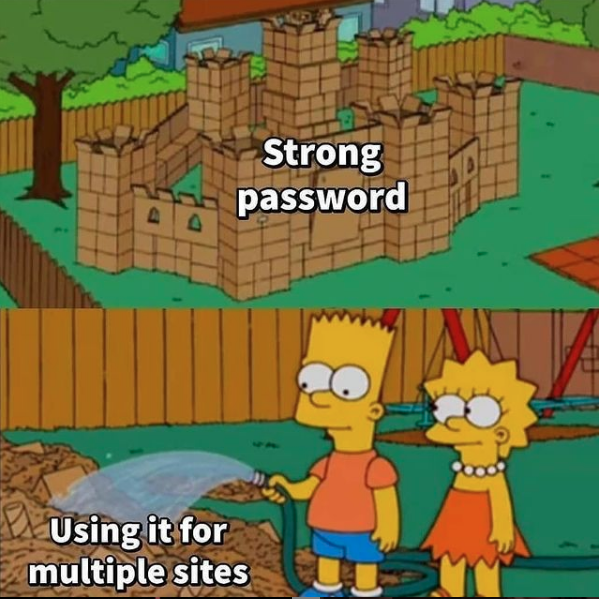
\includegraphics[width=90mm]{Immagini/9/simpson.png}
\end{figure}

\newpage

\subsection{10 Comandamenti del Hash Cracking}

\begin{enumerate}

    \item Conoscerai i tipi di hash e la loro origine/funzione
    \item Conoscerai i punti di forza e di debolezza dei software di cracking
    \item Studierai e applicherai tecniche di analisi delle password
    \item Devi essere esperto nei metodi di estrazione dell'hash
    \item Creerai dizionari personalizzati/mirati
    \item Conoscerai le capacità delle tue piattaforme di cracking
    \item Comprenderai la psicologia/comportamento umano di base
    \item Creerai maschere, regole personalizzate
    \item Sperimenterai continuamente nuove tecniche
    \item Sosterrai i tuoi compagni di cracking membri della comunità

\end{enumerate}
